\subsubsection{Marsch „In Treue fest!“}

 Der Marsch „In Treue fest!“ ist
August Högns einzige im Druck erschienene Komposition. Er wurde deshalb
in den Bestand der Bayerischen Staatsbibliothek aufgenommen. Weder in
Ruhmannsfelden noch bei Högns Nachkommen war ein Exemplar der
gedruckten Fassung für Klavier zu zwei oder vier Händen aufzufinden.
Wer aus diesem Umstand Zweifel an der Urheberschaft Högns anbringen
will und einen Namensvetter als Komponist für wahrscheinlicher hält,
kann mit einer Reihe von Hinweisen, die alle für Högn als Komponist des
Marsches sprechen, überzeugt werden. Orts- und Zeitangaben
(Wallersdorf, 1905) auf dem Titelblatt stimmen zur entsprechenden Zeit
mit dem Wohnort Högns überein. Der Marsch ist der niederbayerischen
Lehrerschaft gewidmet, also dem Lehrerverband, bei dem August Högn 60
Jahre Mitglied war. \footnote{Dokument Nr. 51, Zeitungsartikel aus
Viechtacher Bayerwald-Bote, 15.12.1961} Einzelne fragmentarisch
erhaltene Stimmen eines Arrangements für Orchester, das Högn
handschriftlich angefertigt, schließlich verworfen und als
Papierlieferant für geistliche Kompositionen verwendet hat, sind
schließlich der unumstößlichste Beweis der Urheberschaft. Wie die
Widmung andeutet, könnte der Marsch bei Veranstaltungen des
Lehrerverbands aufgeführt worden sein. In der Orchesterfassung war er
höchst wahrscheinlich ein Repertoirestück des Turnverein-Orchesters und
kam bei vom Turnverein veranstalteten „bunten Abenden“ zum Klingen.

\begin{center}
\begin{minipage}{5.884cm}
\begin{flushleft}
\tablefirsthead{}
\tablehead{}
\tabletail{}
\tablelasttail{}
\begin{supertabular}{m{5.684cm}}

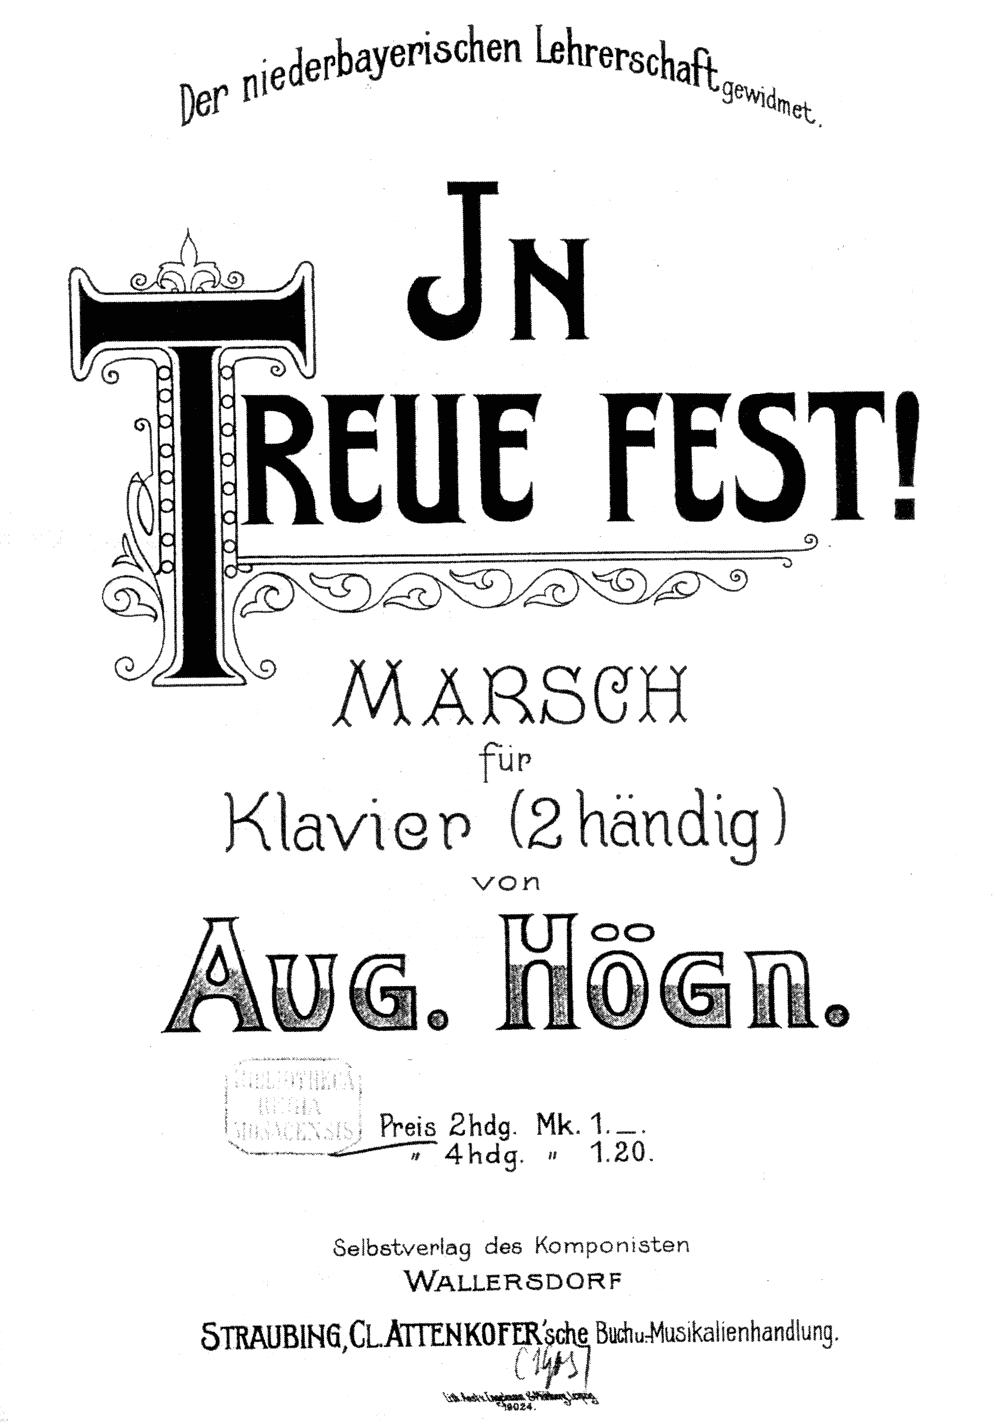
\includegraphics[width=5.503cm,height=7.862cm]{pictures/zulassungsarbeit-img104.png}

Titelblatt des Marsches „In Treue
fest!“\\
\end{supertabular}
\end{flushleft}
\end{minipage}
\end{center}
\begin{center}
\tablefirsthead{}
\tablehead{}
\tabletail{}
\tablelasttail{}
\begin{supertabular}{m{10.502cm}}

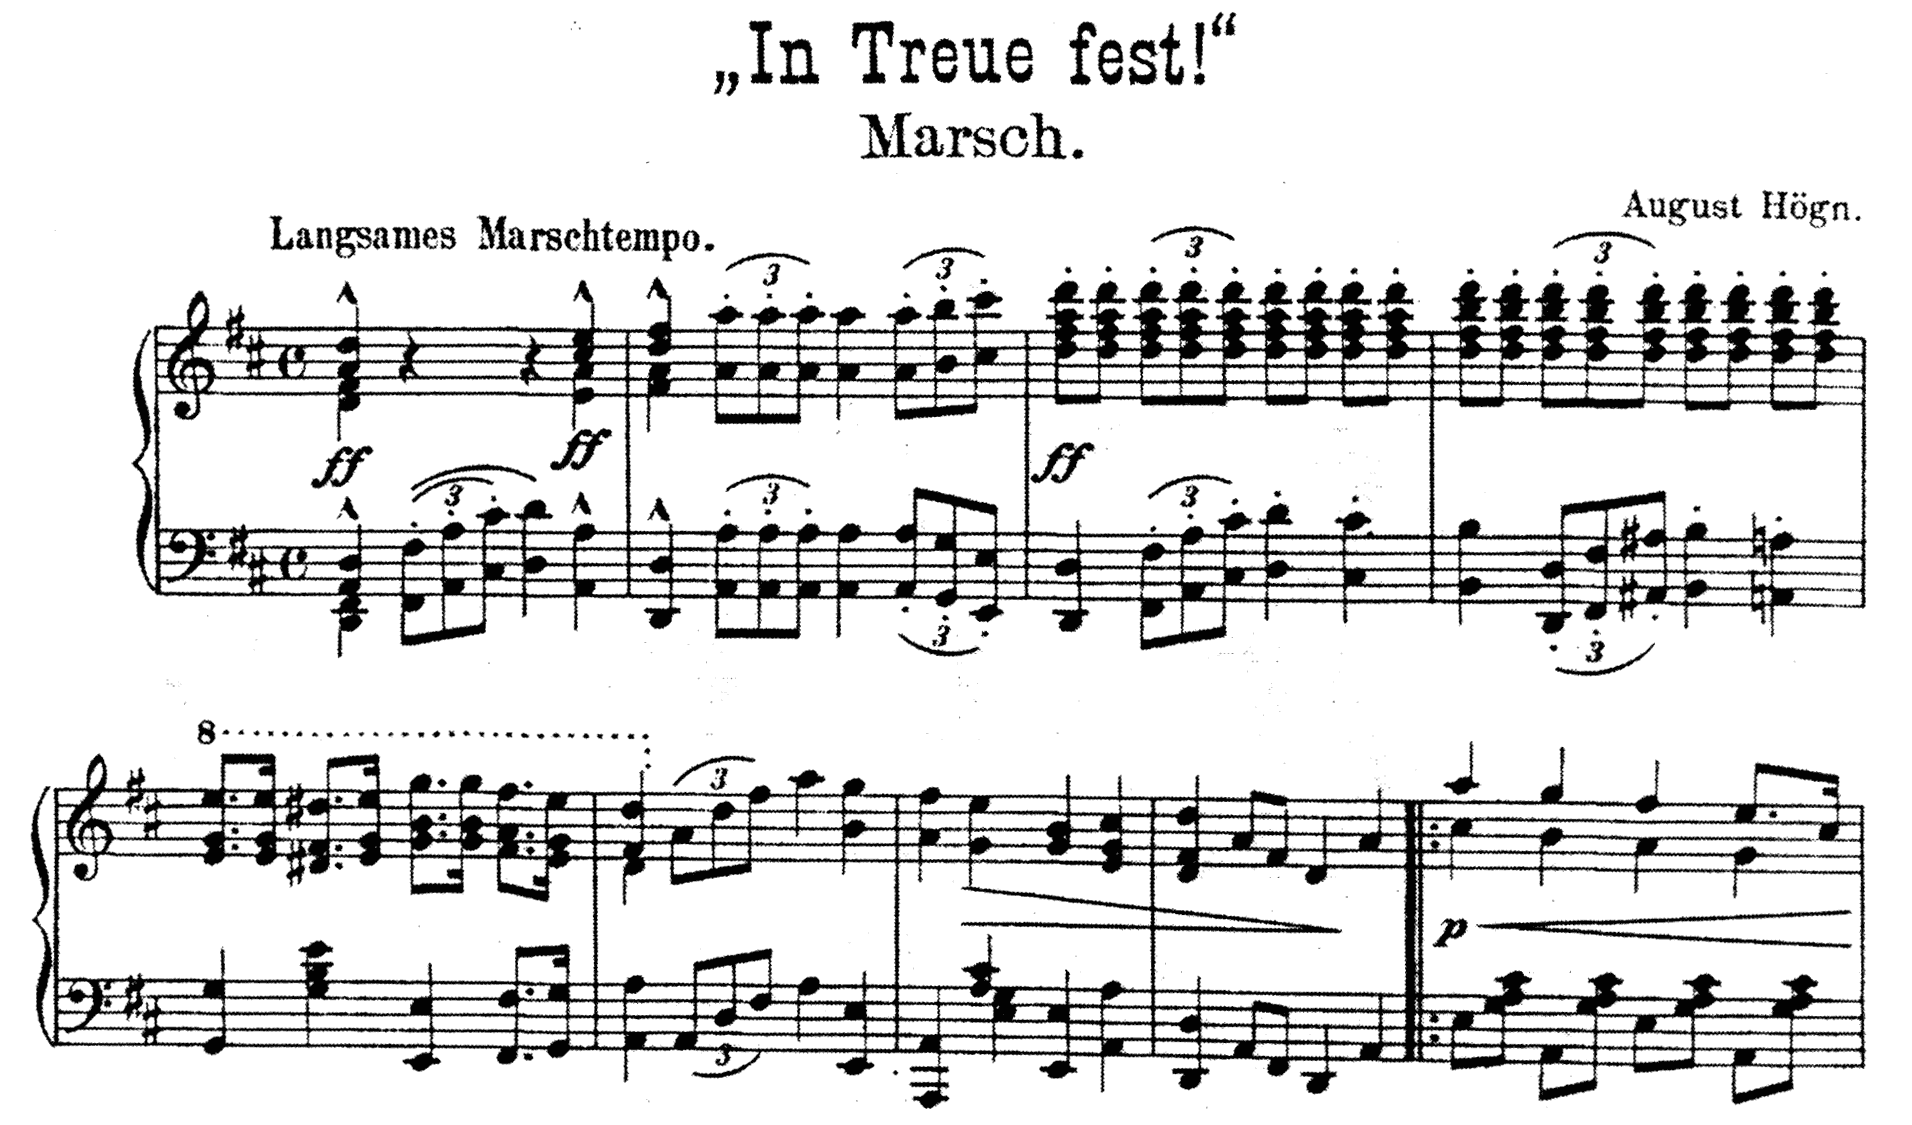
\includegraphics[width=10.319cm,height=6.071cm]{pictures/zulassungsarbeit-img105.png}

Marsch „In Treue fest!“ Einleitung\\
\end{supertabular}
\end{center}
Als besonders gelungen kann die Introduktion des Marsches (siehe auch
Band III, Seite 96 – 97) bezeichnet werden. Zum einen verleihen die
fanfarenartigen aufsteigenden Dreiklangsbrechungen im Bassregister der
Einleitung (Takt 1, 3 und 4) einen erhabenen und zugleich mitreißenden
Charakter, zum anderen werden in der Einleitung gerade die Elemente
vorweggenommen, die im Hauptteil und im Trio Abwechslung vom
schematischen Aufbau des Marsches schaffen. Das direkte
Aufeinanderfolgen verschiedener rhythmischer Modelle – ein Baustein,
durch den der Marsch sehr an Lebendigkeit gewinnt – tritt in der
Einleitung in Form von unmittelbar auf Duolen folgenden Tirolen der
Takte 3 und 4 auf. Die Gegenüberstellung von Triolen und Quartolen in
den Takten 17 – 18 und 21 – 22 scheint dieses Bauprinzip aufzunehmen
und noch zu steigern. Auch das Aufeinandertreffen von Motiven mit
Sechzehntelpunktierungen und dem triolischen Fanfaren-Motiv in mehreren
Takten (z. B. Takt 10 ff.) trägt maßgeblich zur rhythmischen
Mehrschichtigkeit und damit zum aufgelockerten Satzbild bei. Harmonisch
wird das Stück maßgeblich durch die Ausweichungen nach Moll bereichert.
Auch in dieser Hinsicht hat die Introduktion durch seine Ausweichung
nach e-moll Modellcharakter für den Hauptteil und das Trio. Neben den
abschließenden Kadenzvorgängen der ersten zwei Abschnitte des
Hauptteils in den Takten 15 und 24, die e-moll als II: Stufe verwenden,
bietet vor allem die in Moll gehaltene zweite Hälfte des ersten
Trioteils (Takt 32 – 34) eine willkommene Abwechslung zum im Marsch
dominierenden Dur.

Die Ausschmückung des Marsches mit vielen Dynamikwechseln ist ebenso als
eine Maßnahme zur Ablenkung vom immer gleich bleibenden Harmonieschema
anzusehen. Das acht Takte lange Schema – dreimal wiederholt sich ein
dominantisch harmonisierter Takt im Wechsel mit einem tonikalen Takt,
ehe im 7. und 8. Takt eine\newline
II-V-I Kadenz stattfindet – wirkt deswegen so ermüdend, weil es im
Verlauf des Marsches mehrmals wiederholt wird. Es beziehen sich sowohl
der erste als auch der zweite Abschnitt des Hauptteils auf dieses
Schema. Der zweite Abschnitt des Hauptteils wirkt deshalb eher wie eine
Variation des ersten Abschnitts, als ein eigenständiger Formteil.